\section{DFG: discrete feature growth on the toy targets (Part 6)}\label{sec:dfg}

\subsection{The learner}\label{sec:dfgalg}

DFG keeps what Parts 1--5 found the networks to do, and replaces how they search (\cref{tab:dfgmap}). It works with the residual $r=y-\hat y$ of a least-squares fit of the labels on the current features, and with its root mean square $s=\mathrm{rms}(r)$. Training repeats rounds until nothing is accepted, or until the fit already has every training label's sign right.

\paragraph{Candidate classes.} Each class has its own size $N$, and its test uses a union bound over that class.
\begin{itemize}
\item \emph{Global:} every character $\chi_S$ with $|S|\le K$ over all $d$ inputs, so $N=\binom{d}{|S|}$. $K=4$ in the first round and 3 after. Degrees 5 and 6 are also searched in the first round, on a subsample whose size the compute budget sets.
\item \emph{Extension:} $S\cup\{j\}$ and $S\cup\{j,l\}$ for current features $S$.
\item \emph{Local:} every $S$ inside the set $V$ of inputs used by current features, for $|V|\le12$. This is a Walsh transform on $V$, up to completing the junta.
\end{itemize}
The extension and local classes are much smaller than the global one, so features on inputs already in use pass a lower threshold. This is the discrete form of the composition effect of Part 4.

\paragraph{The test.} A candidate is accepted if
\begin{equation}\label{eq:dfgtest}
\Bigl|\tfrac1n\textstyle\sum_{t} r_t\,\chi_S(x_t)\Bigr|\;>\;c\,s\,\sqrt{2\ln(4KN/\delta)/n},\qquad c=1,\ \delta=0.1,\ K=4.
\end{equation}
Everything that passes in a round is added. Since $s$ falls as features are fitted, weaker features become detectable later; this is the noise-limited greedy growth of Parts 1--5.

\paragraph{Block moves.} These are for signal spread over many small coefficients that no single test sees.
\begin{itemize}
\item \emph{Linear block:} all $d$ inputs at once, when a $\chi^2_d$ test on the linear coefficients of the residual rejects at level $\delta$. This is the analogue of the networks' kernel background.
\item \emph{Spectral block:} the top eigen-directions $u$ of the residual pair matrix $\tfrac1n\sum_t r_t x_tx_t^\top$ (diagonal removed) whose eigenvalue clears the noise edge $2s\sqrt{d/n}$. It is used only for $n\ge4d$, and adds the features $(u\cdot x)^2-|u|^2$. It was designed for targets such as MAJ$_5\oplus$MAJ$_5$.
\end{itemize}

\paragraph{Readout and small $n$.}
\begin{itemize}
\item \emph{Readout:} DFG predicts the sign of the least-squares fit, plus one Hebbian step on the residual over all $d$ inputs (the ``kernel background''). Least squares is kept to $p\le n/2$ features, so it never sits at its interpolation peak.
\item \emph{v1.1 refinement:} the least-squares weights are refined by 15 Newton steps of L2-regularized logistic regression ($\lambda=10^{-4}$) when $n\ge8p$.
\item \emph{Forced variant:} with few points the union bound passes nothing; at $n=16$ even a perfect one-input target fails it. For $n\le512$, a ``forced'' variant takes the best-scoring global character anyway, at most twice. It is chosen over the default only if it wins a paired (McNemar) test in cross-validation.
\end{itemize}

\paragraph{Budget.} Each exhaustive search runs on the first $m$ training points, with $m$ set so that it stays within a fixed share of one network run:
\begin{itemize}
\item degree 4: 15\% (25\% in v1);
\item degree 3, and the extensions: 3\% per round each;
\item degrees 5 and 6: 3\% each.
\end{itemize}
Searches whose $m$ would fall below 32 are skipped (v1.1), and degrees 5--6 are skipped below $m=64$. A new round starts only below 75\% of the budget. At $d=30$ the budget binds only for degrees 5--6 ($m\approx1400$ and 150). At $d=60$ and 120 it binds for degree 4 too ($m\approx2200$ and 360).

\paragraph{What is discrete.} The hypothesis is a set of parities $\chi_S$ plus, on dense targets, a few quadratic forms. They are found by enumeration and admitted by explicit tests. The only continuous parameters are the readout weights; the spectral directions $u$ are the one borderline case (\cref{sec:discreteness}).

\begin{table}[t]
\centering\footnotesize
\begin{tabularx}{\linewidth}{>{\raggedright\arraybackslash}X>{\raggedright\arraybackslash}X}
\toprule
what the networks were seen to do (Parts 1--5) & DFG's discrete counterpart\\
\midrule
grow features greedily, in bundles, in order of detectability (plateaus and drops) & rounds of exhaustive search; everything that passes the test this round is added\\
a feature's cost is set by its correlation with the residual against the noise of competing directions & the test \eqref{eq:dfgtest}, with $s=\mathrm{rms}(r)$ and $N$ the size of the candidate class\\
features on a term's own inputs make it cheaper (composition, Part 4) & small candidate classes: extensions $S\cup\{j\}$, $S\cup\{j,l\}$ and local subsets of the inputs in use\\
a kernel background plus a few grown features & a linear block ($\chi^2_d$ test) and a final Hebbian step on the residual\\
dense targets: one direction grown from many weak correlations & a spectral block: eigen-directions of the residual pair matrix above the noise edge\\
on every plateau, the sign of a truncated Fourier expansion & readout: sign of the least-squares fit on the grown features (v1), refined by logistic regression (v1.1)\\
\bottomrule
\end{tabularx}
\caption{How DFG's components map to what Parts 1--5 found the networks to do \cite{gdcircuit2026}.}
\label{tab:dfgmap}
\end{table}

\subsection{Why exhaustive enumeration pays about \texorpdfstring{$\ln N$}{ln N} in samples}\label{sec:lnN}

\begin{remark}[\status{Heuristic}]\label{rem:lnN}
Let $\rho$ be a character's correlation with the current residual, in units of $s$. The left side of \eqref{eq:dfgtest} then concentrates around $\rho s$, with noise of order $s/\sqrt n$. The threshold is the union-bound level over $N$ candidates, so the character is admitted, and no null candidate is, once roughly
\[
n\;\gtrsim\;2\ln(4KN/\delta)/\rho^2 .
\]
For a $k$-sparse character found by the global search, $N=\binom dk\le d^k$, so the sample cost is about $2k\ln d/\rho^2$; this is the Occam rate. The compute cost is about $n\binom dk$ per search.

The networks pay the other way round. Part 3's heuristic law \cite{gdcircuit2026}, fitted to them, has $\nstar\approx c\,N(k)/\rho^2$ with $N(k)=d\max(1,d/a)^{k-2}$, which is about $d^{k-1}$ for a $k$-parity. The measured exponents are 1.0, 1.9 and 2.4 for $k=2,3,4$, and $k=4$ is also limited by the networks' step budget. Under the networks' own FLOP budget, exhaustive search is affordable at $d=30$ up to degree 4 on all the data, and up to degree 6 on a subsample.
\end{remark}

So, heuristically, gradient descent spends data where exhaustive search spends FLOPs. This reading is consistent with the results below but not tested by them. Search is also not the only difference between the two learners. DFG's dictionary, characters on the uniform cube, is the class the targets were built from, and these experiments do not separate the two effects. DFG is in effect a greedy, budgeted form of the classical low-degree algorithm, designed for this function class. The networks are generic and use one untuned configuration.

\subsection{Versions and what is blind}\label{sec:dfgversions}

\begin{itemize}
\item \textbf{v1} (commit \texttt{359a6b61}) is the version run blind on \code{dlheld}.
  \begin{itemize}
  \item \emph{Exception 1.} Its degree-5/6 search was added knowing that $\chi_5$ (par5) was in the suite, and par5's result depends on it entirely. The blind row therefore uses v1 without that search ($K_{\rm hi}=4$).
  \item \emph{Exception 2.} The spectral block was committed together with the suite, and its docstring works through MAJ$_5\oplus$MAJ$_5$, which is the suite's majxor.
  \end{itemize}
\item \textbf{v1.1} (\texttt{0220cf04}) was made after that run. It fixes two problems.
  \begin{itemize}
  \item \emph{The readout.} On the dense halfspace thr30, v1's least-squares readout plateaued at 5--7\% error, where the networks reach 1\%. The logistic refinement takes thr30's error from 0.054 to 0.010 (post hoc).
  \item \emph{A budget bug found by the compute audit.} v1's small-$n$ cross-validation gave every fold the whole budget. At $d=120$ that cost up to 2.7 runs of a 20000-step network per fit. v1.1 splits the budget across folds and adds a 0.75 hard cap.
  \end{itemize}
  v1.1 also skips searches with $m<32$. That rule is why its $\nstar$ for par3 and par4 at $d=30$ (28 and 52) are higher than v1's (16 and 21).
\item \textbf{\code{dlheld2}} was committed after v1.1 (\texttt{70c604eb}), and DFG's code was not changed afterwards except for its name and an input-permutation wrapper. So that suite is blind for v1.1. It was written by DFG's designer, mostly from families already in the development suites, so it is blind to tuning, not to the choice of targets.
\item \textbf{The development suites are in-sample.}
  \begin{itemize}
  \item \code{designed}: DFG's settings, notably the small-$n$ rules and the $n\ge4d$ gate on the spectral block, were chosen by looking at its test error there.
  \item \code{random}: it was run twice with intermediate versions and read.
  \end{itemize}
\end{itemize}

\subsection{Results against the networks}\label{sec:dfgresults}

\begin{table}[t]
\centering\footnotesize\setlength{\tabcolsep}{3.5pt}
\begin{tabular}{lcccccc}
\toprule
suite, DFG version & clearly better & clearly worse & median & geo.\ mean & cells worse by $>0.02$ ($>2$ s.e.) & max FLOPs / run\\
\midrule
\code{dlheld2} (7), v1.1, permuted --- \textbf{blind} & 7 & 0 & 3.1$\times$ & 3.4$\times$ & 6 (3) of 77 & 0.26\\
\code{dlheld} (12), v1 without deg.\ 5--6 --- \textbf{blind} & 11 & 1 & 2.7$\times$ & 3.7$\times$ & 13 (12) of 132 & 0.17\\
\code{dlheld} (12), v1 (deg.\ 5--6 added knowing par5) & 12 & 0 & 2.8$\times$ & 5.2$\times$ & 11 (10) of 132 & 0.23\\
\code{dlheld} (12), v1.1 --- post hoc & 12 & 0 & 3.0$\times$ & 5.3$\times$ & 6 (5) of 132 & 0.43\\
\code{random} (20), v1 --- development & 20 & 0 & 6.0$\times$ & 6.8$\times$ & 9 (5) of 220 & 0.14\\
\code{designed} (21), v1 --- in-sample & 20 & 0 & 5.4$\times$ & 7.0$\times$ & 7 (2) of 231 & 0.19\\
\code{designed} at $d=15$ (7), v1 & 7 & 0 & 6.0$\times$ & 6.3$\times$ & 1 (0) of 77 & 0.08\\
\code{designed} at $d=60$ (7), v1.1 & 7 & 0 & 31.7$\times$ & 36.3$\times$ & 0 (0) of 77 & 0.46\\
\code{designed} at $d=120$ (4), v1.1 & 4 & 0 & 45.5$\times$ & 30.7$\times$ & 0 (0) of 29 & 0.18\\
\bottomrule
\end{tabular}
\caption{DFG against the study's networks \status{Numerical}. The median and geometric-mean data factors are the networks' $\nstar$ over DFG's, over targets both learn. ``Cells'' are $(\text{target},n)$ pairs on the 11-point grid where DFG's seed-mean error exceeds the networks' by more than 0.02 (in brackets: also by more than 2 s.e.\ of the seed spread). The last column is DFG's largest per-fit compute as a fraction of one network run. Source: \repo{study/discrete_learner/RESULTS.md}.}
\label{tab:dfgsummary}
\end{table}

\begin{figure}[t]
\centering
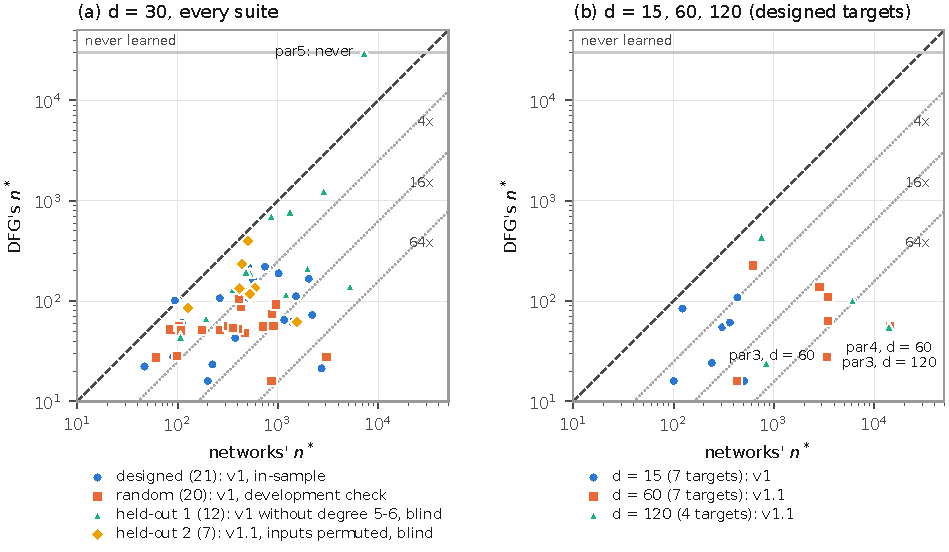
\includegraphics[width=\linewidth]{figures/fig_dfg_nstar.pdf}
\caption{DFG's $\nstar$ against the networks' $\nstar$, one point per target, on log axes. Points below the dashed diagonal are targets where DFG needs less data; the dotted lines mark 4, 16 and 64 times less. (a) $d=30$: the two blind runs (\code{dlheld} with frozen v1 without its degree-5/6 search, and \code{dlheld2} with v1.1 on permuted inputs) and the development suites (v1, natural input order). par5, which DFG never learns without the degree-5/6 search, is drawn at the top. (b) The designed targets run at $d=15$ (v1), 60 and 120 (v1.1). The par4 point at $d=60$ and the par3 point at $d=120$ coincide.}
\label{fig:dfgnstar}
\end{figure}

\Cref{tab:dfgsummary} and \cref{fig:dfgnstar} summarize the comparison \status{Numerical}.

\paragraph{Blind tests.}
\begin{itemize}
\item \emph{\code{dlheld2}, the final version.} DFG v1.1 has the smaller $\nstar$ on all 7 targets: median factor 3.1, geometric mean 3.4, with at most 0.26 of a network run per fit. The smallest gains are on the symmetric sym8 (1.3$\times$), the random formula h2rf1 (1.5$\times$) and the 2-DNF (1.9$\times$). sym8's is marginal across seeds.
\item \emph{\code{dlheld}, frozen v1 without its degree-5/6 search.} DFG has the smaller $\nstar$ on 11 of 12 targets, by a median factor of 2.7. Without that search it has no route to a degree-5 character, so it never learns par5, while the networks learn it at $n\approx7200$.
\end{itemize}

\paragraph{Development suites and input dimension.}
\begin{itemize}
\item \emph{Development suites.} On the 41 targets of \code{designed} and \code{random}, $\nstar$ is clearly smaller on 40. The 41st, and3, is a tie (101 against 94).
\item \emph{Dense targets} (majorities, halfspaces, intersections of halfspaces, MAJ$_5\oplus$MAJ$_5$, sym8): the factor is 1.2--4.4. Heuristically, and with no linear baseline run in Part 6, this is the difference between a well-fitted linear readout and the networks' learned features. Part 8's \code{lin} reference is consistent with this reading (\cref{sec:lin}).
\item \emph{Sparse targets} (parities, staircases, majorities of parities, multiplexers, random formulas): the factor is 1.5--250, growing with $d$.
\item \emph{Parities across $d$.} For par3 the networks need 843, 3410 and about 14000 samples at $d=30$, 60 and 120, and DFG needs 28, 28 and 56. For par4 the networks need 2728 and 14255 at $d=30$ and 60, and DFG needs 52 and 56. These DFG values are from v1.1 with the inputs permuted per fit; the unpermuted runs give the same values.
\item \emph{Caveats on the $d$-scaling rows.} Their targets are in-sample and mostly sparse, so their median rises partly because the target mix changes. For maj9 the factor stays at 1.5--2.7$\times$ across $d$.
\end{itemize}

\paragraph{Where DFG is worse.} Per $(\text{target},n)$ cell, DFG's error exceeds the networks' by more than 0.02 in 0--10\% of cells, depending on the suite. These cells are of three kinds.
\begin{itemize}
\item \emph{$n=16$--64.} Most of the cells are here, where both learners are near the constant predictor's error and DFG is sometimes above it. For example, sym8 at $n=32$ has 0.40 against the networks' 0.34 and the constant's 0.28.
\item \emph{thr30 at $n\ge2048$, in v1:} the least-squares readout plateau.
\item \emph{MAJ$_5\oplus$MAJ$_5$ (majxor) at $n=64$--256}, in both versions.
  \begin{itemize}
  \item The networks are partly there (0.36 at $n=256$), while DFG is at chance until its spectral block fires near $n=512$.
  \item DFG then leads: 0.02--0.03 against 0.16 at $n=1024$.
  \end{itemize}
\end{itemize}
So ``at least as good'' holds for $\nstar$ on every target of the blind tests except par5 without the degree-5/6 search. It does not hold for every cell.

\paragraph{Compute.} DFG uses less compute than a network run everywhere: at most 0.46 of a run per fit, and under 0.08 at $n\le512$ at $d=30$. In recorded CPU time it is comparable at $d=30$ (0.25--1.7$\times$ a network at $n=16384$) and 2--4$\times$ faster at $d=120$. This is despite DFG running in float64 numpy against the networks' float32 XLA (\cref{app:compute}). The claim is about FLOPs.

\paragraph{Tie-break bias and robustness.}\label{sec:tiebreak}
\begin{itemize}
\item \emph{Tie-breaks.} Every suite lists the relevant inputs first, and DFG's enumeration breaks exact ties toward low indices. At $n=16$--32 the forced guess therefore wins ties toward the true target. The reproduction audit measured this on frozen v1: with permuted columns, par4 at $n=16$ goes from 0.17 to 0.40 error and par3 at $n=16$ from 0.00 to 0.13, and the designed suite's mean $\log_2$ ratio moves by about $+0.03$.
\item \emph{Permuted runs.} \code{dlheld2} and the ablations were run with the inputs permuted at random per fit, which removes the bias. The development rows were not.
\item \emph{Fresh seeds.} Fresh training seeds at the grid points bracketing DFG's $\nstar$ reproduce the recorded errors for stair5, rmaj9, parmaj and par3. mux is the exception: on 9 fresh seeds its $\nstar$ is about 87 rather than 65, so its factor is about 13, not 18.
\item \emph{Definition of $\nstar$.} An alternative definition, the smallest grid $n$ from which the error stays at most 0.1, changes the mean $\log_2$ ratios by at most 0.10--0.15.
\end{itemize}

\subsection{Ablations}\label{sec:dfgabl}

\begin{table}[t]
\centering\footnotesize\setlength{\tabcolsep}{4.5pt}
\begin{tabular}{lrrrrrrrr}
\toprule
variant (one ingredient removed) & maj9 & thr10 & par4 & stair5 & mux & rmaj9 & sparsepoly & mean $\log_2$ vs full\\
\midrule
full DFG v1.1 & 107 & 146 & 52 & 111 & 64 & 167 & 93 & $+0.00$\\
global search to degree 3 only & 107 & 152 & never & 113 & 158 & 167 & 93 & $+1.34$\\
raw-coefficient readout & 309 & 295 & 52 & 112 & 63 & 210 & 99 & $+0.42$\\
thresholds scaled by the label, not the residual & 107 & 148 & 56 & 165 & 111 & 188 & 97 & $+0.25$\\
no composition classes & 107 & 142 & 52 & 196 & 107 & 167 & 108 & $+0.25$\\
no background, no small-$n$ variant & 107 & 146 & 52 & 112 & 110 & 167 & 107 & $+0.14$\\
no blocks & 168 & 144 & 52 & 111 & 61 & 178 & 80 & $+0.07$\\
least-squares readout (v1's) & 107 & 170 & 52 & 112 & 65 & 167 & 101 & $+0.05$\\
\midrule
networks & 263 & 563 & 2728 & 1514 & 1156 & 2027 & 2205 & \\
\bottomrule
\end{tabular}
\caption{DFG ablations: $\nstar$ on 7 designed targets, $d=30$, inputs permuted, 3 seeds \status{Numerical}. A target never learned counts $+8$ in the mean. Changes below about $1.2\times$ may be seed noise. Source: \repo{study/discrete_learner/RESULTS.md}.}
\label{tab:dfgabl}
\end{table}

\Cref{tab:dfgabl} removes one ingredient at a time \status{Numerical}.
\begin{itemize}
\item \textbf{Only two ablations lose to the networks}: par4 without the degree-4 search (never learned), and MAJ$_9$ with the raw-coefficient readout (309 against 263). Every other variant stays far ahead.
  \begin{itemize}
  \item By elimination, the gap is plausibly carried by what every variant keeps: exhaustive search over the Fourier dictionary with union-bound tests.
  \item That was not ablated directly, so the attribution is \status{Heuristic}.
  \end{itemize}
\item \textbf{The global search depth decides which leaps are possible.}
  \begin{itemize}
  \item Without degree 4, par4 has no lower-order signal, so neither extensions nor local search can reach it.
  \item mux gets 2.5$\times$ worse, because its term $x_1x_2x_3x_4$ must then be built by extension.
  \item This is the discrete analogue of leap complexity. The difference from the networks is that a leap costs DFG $\ln\binom dk$ in samples and $\binom dk$ in compute, not about $d^{k-1}$ in samples.
  \end{itemize}
\item \textbf{Each ingredient taken from the networks is worth 1.1--3$\times$ on one class of targets.}
  \begin{itemize}
  \item \emph{The readout fitted to the residual}, against raw Fourier coefficients: 2.9$\times$ on MAJ$_9$ and 1.3$\times$ on rmaj9. On thr10 it is worth 1.7$\times$ (295 against 170), and the logistic refinement adds 1.2$\times$ (170 to 146).
  \item \emph{Residual-scaled thresholds}: 1.5$\times$ on stair5 and 1.7$\times$ on mux. These are staged targets, where later terms become detectable only once earlier ones are fitted.
  \item \emph{Composition classes}: 1.8$\times$ on stair5, 1.7$\times$ on mux and 1.2$\times$ on sparsepoly. These are the targets whose high-degree terms sit on the inputs of their low-degree terms. The direction matches the networks' composition effect (Part 4 measured 1.2--1.6$\times$ for them).
  \item \emph{The linear block}: 1.6$\times$ on MAJ$_9$, whose nine inputs would otherwise each need to pass an individual test.
  \end{itemize}
\item \textbf{The blocks cost a little on sparse targets}: sparsepoly goes from 93 to 80 without them.
\end{itemize}

\subsection{Limits}\label{sec:dfglimits}

\begin{itemize}
\item \textbf{A narrow inductive bias.} The dictionary is characters on the Boolean cube plus a few quadratic forms, and the tests rely on characters being orthogonal under the uniform distribution. Other input distributions, real-valued inputs and images need a different dictionary (\cref{sec:standard}).
\item \textbf{Compute grows as $d^K$.} Under a fixed budget DFG subsamples, so a high-degree feature must have a large coefficient to be found. At $d=30$ the degree-6 search sees about 150 points, and degrees 5--6 are skipped at $d\ge60$.
\item \textbf{One network configuration.} The reference is the study's fixed configuration, never tuned, while DFG's settings were tuned on the designed suite. Earlier parts found that the networks' $\nstar$ moves by up to about $2\times$ with width or optimizer. That is below the blind median factor of 3.1, but comparable to the smallest blind wins (1.3--1.9$\times$). Part 8 measured the effect of weight decay and logistic loss directly (\cref{sec:toyresults}).
\end{itemize}
